\chapter[Serviços]{Serviços}

\section{Conceitos básicos}

Com o advento das tecnologias e evoluções no mercado global a busca por qualidade em todos os setores cresceu. A evolução acontece na melhoria de seus processos, equipamentos e pessoas para que a organização tenha vantagem em seu meio de atuação. Essa busca por qualidade reduz retrabalho, reduz perdas e aumenta a satisfação dos consumidores \cite[p.~150]{slack2002}.

A evolução e melhoria na qualidade também aumentou as expectativas dos consumidores, \cite [p.~42]{parasuraman1991} destacam que quanto mais experiente o consumidor, maior sua expectativa da qualidade do serviço. Com a globalização a informação está ao dispor do usuário com facilidade, aumentando o fator de expectativa do serviço, tornando a qualidade um aspecto imprescindível no fornecimento de serviços. Cada serviço tem suas características próprias, porém a maioria compartilha das mesmas propriedades básicas. Para \apud[p.~5]{gronroos1993}{santos2007} a maioria dos serviços possuem quatro propriedades básicas:
\begin{itemize}
	\item Os serviços são mais ou menos intangíveis;
	\item Os serviços são atividades ou uma série de atividade em vez de coisas;
	\item Os serviços são, pelo menos até certo ponto, produzidos e consumidos simultâneamente;
	\item O cliente participa do processo de produção, pelo menos até certo ponto.
\end{itemize}


Portanto, o controle de qualidade é um fator complexo de se gerenciar, pois não há pré-qualidade comprovada para ser comercializada e o serviço é produzido enquanto é consumido.

\cite[p.~47]{gronroos1993} também alega que muitas empresas sentem dificuldade em gerenciar com efetividade seu controle de qualidade, pois se preocupam com os fatores internos de suas organizações e os consumidores e suas percepões não são incluídas nas medições de qualidade, o que torna o índice avaliado restrito à qualidade interna da organização.

Com as dificuldades citadas, o próximo capítulo traz as características da avaliação que devem suprir a dificuldade do controle de qualidade. Tais características geram necessidade de atividades que precisam ter abordagens específicas para que se tenha a avaliação correta destes serviços. 

\subsection{Qualidade de serviço}

As características supracitadas dos serviços os torna mais difíceis de serem avaliados do que os produtos, pois em um produto tangível, os consumidores podem visualizar suas características antes de comprar. A importância da avaliação correta dos serviços, é saber o que satisfaz as expectativas e necessidades dos consumidores. O levantamento correto dessas necessidades e as ações com o consumidor em foco, garantem a sobrevivência econômica da organização \cite{zeithaml1981}. 

Mas, a qualidade deve ser definida antes de sabermos o que deve ser levantado. \cite{garvin1984} definiu 5(cinco) abordagens para qualidade, são elas:
\begin{itemize}
	\item Abordagem transcendental, na qual a qualidade é uma excelência inata. Absoluta e universalmente reconhecível, um indício de padrões elevados e altas conquistas. Porém, é uma característica que é reconhecida somente pela experiência, tornando sua quantificação difícil de analisar precisamente;

	\item Abordagem baseada no produto, na qual a qualidade é uma variável precisa e mensurável. As diferenças na qualidade refletem diferentes quantidades de alguns atributos ou ingredientes de algum produto. Como por exemplo, o ar de boa qualidade pode ser considerado de boa qualidade se tiver um grau baixo de poluentes por $m^3$. Para produtos a qualidade pode ser definida pela quantidade de um atributo ou característica desejada, porém, uma análise livre de erros só é possível se o atributo em questão é considerado preferível, virtualmente, por todos os consumidores;

	\item Abordagem baseada no usuário, na qual a qualidade "está nos olhos de quem vê". Individualmente, os consumidores são muito diferentes, portanto algo que melhor satisfaça suas necessidades ou expectativas é considerado como de alta qualidade, porém, é uma abordagem com uma visão altamente subjetiva, tornando difícil sua quantificação com exatidão;
	
	\item Abordagem baseada em manufatura, na qual o foco está na parte fornecedora, a maior preocupação está no processo e engenharia de manufatura onde a qualidade é identificada como conformidade aos requisitos. Assim que um padrão é definido, qualquer mudança ou desvio desse padrão é considerado como diminuição da qualidade;

	\item Abordagem baseada em valores, na qual a qualidade é definida na precificação, custos e preços. Nessa visão, algo com qualidade deve ter uma performance aceitável por um preço aceitável ou conformidade a um custo aceitável. A dificuldade dessa visão está na relação de dois conceitos relacionados porém distintos, qualidade e valor financeiro. O resultado dessa mistura é uma excelência financeira que dificulta a definição pura da qualidade.
\end{itemize}

Segundo \cite{paladini1995} quando uma organização se preocupa com a abordagem baseada no usuário há uma tendência de acoplar as preocupações com as outras abordagens, se tornando assim, uma definição de qualidade mais completa, pois quando há uma preocupação com valores, atributos desejáveis, conformidades com os requisitos e marca, define-se a preocupação com as necessidades do consumidor. Portanto o foco deste trabalho se valhe da abordagem baseada, principalmente, na ótica do consumidor, neste caso, o cidadão.

\subsection{Dimensões de avaliação da qualidade}

Como dito na seção anterior os serviços tem características únicas que os diferem dos bens físicos na relação serviço versus produto. Essas peculiaridades dificultam a garantia de satisfação do cliente, visto que a dificuldade de controle e a segurança da garantia de qualidade são complexas de se assegurar. As diferentes características de serviços e produtos são mostrados na Tabela \ref{table:diferencas} \cite{gronroos1993}.

% Please add the following required packages to your document preamble:
% \usepackage[table,xcdraw]{xcolor}
% If you use beamer only pass "xcolor=table" option, i.e. \documentclass[xcolor=table]{beamer}
\begin{table}[!h]
\centering
\caption{Diferenças entre serviços e bens físicos. Adaptado de \cite{gronroos1993}}.
\label{table:diferencas}
\resizebox{.6\textwidth}{!}{%
\begin{tabular}{|c|c|}
\hline
\rowcolor[HTML]{C0C0C0} 
{\color[HTML]{343434} BENS FÍSICOS} & {\color[HTML]{343434} SERVIÇOS} \\ \hline
Tangível & Intangível \\ \hline
Homogêneo & Heterogêneo \\ \hline
\begin{tabular}[c]{@{}c@{}}Produção e distribuição\\ separadas do consumo\end{tabular} & \begin{tabular}[c]{@{}c@{}}Produção, distribuição e \\ consumo são processos \\ simultâneos\end{tabular} \\ \hline
Um artefato tangível & Uma atividade ou processo \\ \hline
\begin{tabular}[c]{@{}c@{}}Valor principal produzido em\\ fábricas\end{tabular} & \begin{tabular}[c]{@{}c@{}}Valor principal produzido nas\\ interações entre comprador e vendedor\end{tabular} \\ \hline
\begin{tabular}[c]{@{}c@{}}Clientes não participam do\\ processo de produção\end{tabular} & Clientes participam na produção \\ \hline
Pode ser mantido em estoque & \begin{tabular}[c]{@{}c@{}}Não pode ser mantido em\\ estoque\end{tabular} \\ \hline
Transferência de propriedade & Não transfere propriedade \\ \hline
\end{tabular}
}
\end{table}

Vários autores tiveram visões diferentes sobre quais são os fatores determinantes na avaliação de qualidade em serviços. Na Tabela \ref{table:determinantes} \cite{bouranta2009} podemos ver uma compilação desses fatores e seus idealizadores.

\nopagebreak
\begin{table}[!h]
\centering
\caption{Determinantes de avaliação da qualidade em serviços. Adaptado de \cite{bouranta2009}.}
\label{table:determinantes}
\resizebox{\textwidth}{!}{%
\begin{tabular}{|l|l|l|l|l|l|l|l|l|}
\hline
\multicolumn{1}{|c|}{\begin{tabular}[c]{@{}c@{}}Determinantes\\ da qualidade\\ em serviços\end{tabular}} & \multicolumn{1}{c|}{\begin{tabular}[c]{@{}c@{}}Parasuraman et al.\\ (1985)\end{tabular}} & \multicolumn{1}{c|}{\begin{tabular}[c]{@{}c@{}}Gremler et al.\\ (1994)\end{tabular}} & \multicolumn{1}{c|}{\begin{tabular}[c]{@{}c@{}}Brooks et al.\\ (1999)\end{tabular}} & \multicolumn{1}{c|}{\begin{tabular}[c]{@{}c@{}}Reynoso\\ \& Moores\\ (1995)\end{tabular}} & \multicolumn{1}{c|}{\begin{tabular}[c]{@{}c@{}}Gianesi\\ \& Corrêa\\ (1996)\end{tabular}} & \multicolumn{1}{c|}{\begin{tabular}[c]{@{}c@{}}Marshall et al.\\ (1998)\end{tabular}} & \multicolumn{1}{c|}{\begin{tabular}[c]{@{}c@{}}Paraskevas\\ (2001)\end{tabular}} & \multicolumn{1}{c|}{\begin{tabular}[c]{@{}c@{}}Yeh et al.\\ (2007)\end{tabular}} \\ \hline
Tangibilidade & \checkmark &  &  & \checkmark & \checkmark &  &  & \checkmark \\ \hline
Cofiabilidade & \checkmark &  & \checkmark & \checkmark & \checkmark &  &  & \checkmark \\ \hline
Presteza & \checkmark & \checkmark & \checkmark & \checkmark & \checkmark &  &  & \checkmark \\ \hline
Garantia & \checkmark &  &  &  &  &  &  &  \\ \hline
Credibilidade & \checkmark &  & \checkmark &  &  &  &  & \checkmark \\ \hline
Competência & \checkmark &  & \checkmark & \checkmark & \checkmark &  & \checkmark & \checkmark \\ \hline
Cortesia & \checkmark &  & \checkmark & \checkmark &  & \checkmark &  & \checkmark \\ \hline
Empatia & \checkmark &  &  &  &  &  &  &  \\ \hline
Comunicação & \checkmark &  & \checkmark & \checkmark &  &  & \checkmark & \checkmark \\ \hline
Compreensão & \checkmark &  & \checkmark & \checkmark &  &  & \checkmark & \checkmark \\ \hline
Acessibilidade & \checkmark &  & \checkmark &  & \checkmark &  &  & \checkmark \\ \hline
Segurança & \checkmark &  &  &  & \checkmark &  &  &  \\ \hline
Flexibilidade &  & \checkmark &  & \checkmark & \checkmark &  & \checkmark &  \\ \hline
Proatividade &  &  & \checkmark & \checkmark &  &  &  &  \\ \hline
Liderança &  &  & \checkmark &  &  &  &  &  \\ \hline
\end{tabular}%
}
\end{table}

Com os fatores determinantes da qualidade em mãos, surgiram os modelos de avaliação de qualidade, os quais serão abordados nas próximas seções.

\newpage
\section{SERVQUAL: Modelo de avaliação da qualidade de serviço}

\subsection{Concepção do modelo}
Os trabalhos de Parasuraman, Zeithaml e Berry se destacam por se tratar de avaliação de qualidade do ponto de vista do cliente, eles ressaltam um modelo denominado SERVQUAL\cite{parasuraman1985}. Os autores definem um modelo baseado em lacunas para aferição da qualidade. São 5 lacunas entre percepções e expectativas do usuário ou cliente do serviço e o que é entregue e percebido pelos fornecedores desses serviços, a Imagem \ref{img:modelodequalidade} mostra o modelo proposto.
\begin{center}
	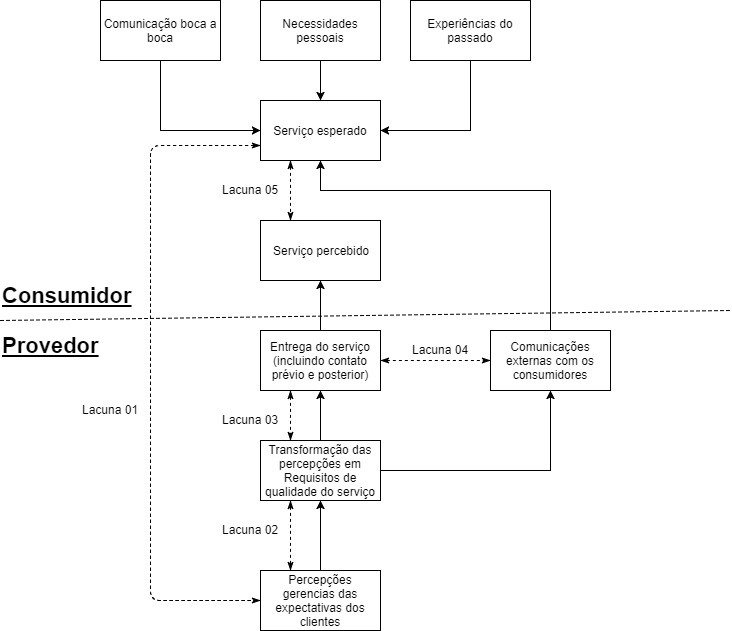
\includegraphics[width=.75\linewidth]{figuras/modelodequalidade.jpg}
	\captionof{figure}{Modelo de Qualidade de serviços. Adaptado de \cite{parasuraman1985}}.
	\label{img:modelodequalidade}
\end{center}

As lacunas são analisadas pelos autores e em cada uma delas há uma proposição sobre seus impactos:
\begin{itemize}
	\item \textbf{Lacuna 01 - Percepção e gerenciamento da expectativa do cliente}: Esta lacuna, entre as expectativas dos consumidores e gerenciamento das percepções da empresa sobre essas expectativas, terá impacto direto na avaliação do consumidor sobre a qualidade do serviço;
	\item \textbf{Lacuna 02 - Gerenciamento da percepção e especificação da qualidade do serviço}: Esta lacuna entre o gerenciamento das percepções dos consumidores e as especificações próprias da qualidade afetarão a qualidade do serviço no ponto de vista do consumidor;
	\item \textbf{Lacuna 03 - Especificações da qualidade do serviço e a entrega do serviço}: A lacuna entre as especificações de qualidade do serviço e a entrega do serviço afetarão a qualidade do serviço no ponto de vista do consumidor;
	\item \textbf{Lacuna 04 - Entrega do serviço e comunicações externas}: Esta lacuna também afetará como o consumidor avalia a qualidade do serviço;
	\item \textbf{Lacuna 05 - Serviço esperado e o serviço percebido}: A qualidade que o consumidor percebe em um serviço é a função de magnutide e direção da lacuna entre o serviço esperado e o percebido.
\end{itemize}

\subsection{Instrumento: Dimensões e questões}
Os autores, então, desenvolveram um questionário para continuação do trabalho que haviam desenvolvido. Este questionário tinha como base os determinantes para a avaliação da qualidade dos serviços e foi chamado de SERVQUAL. 

Como podemos ver, há uma divisão na Imagem \ref{img:modelodequalidade} onde existe uma lacuna que identifica a qualidade recebida e a percebida, que incluiriam todas as outras 4 (quatro) lacunas. O SERVQUAL também seguiu essa linha de raciocínio e foi dividido em duas partes: uma para análise da qualidade percebida e outro para a avaliação da qualidade esperada. Ao todo o questionário contava com 97 (noventa e sete) questões, mas nas fases de validação do instrumento e análise das dimensões que o modelo avaliava as questões foram reduzidas a 22 (vinte e duas) \cite{parasuraman1988}.

As 22 (vinte e duas) questões avaliavam 5 (cinco) dimensões relacionadas na Tabela \ref{table:consistenciainterna} \cite{parasuraman1988}. As questões de cada dimensão podem ser visualizadas na Tabela \ref{table:servqualquestoes} \cite{parasuraman1988}.

\begin{table}[]
\centering
\caption{Dimensões avaliadas pelo SERVQUAL \cite{parasuraman1988}.}
\label{table:consistenciainterna}
\begin{tabular}{|c|c|c|}
\hline
\rowcolor[HTML]{C0C0C0} 
Dimensão & \begin{tabular}[c]{@{}c@{}}Descrição da \\ dimensão\end{tabular} & \begin{tabular}[c]{@{}c@{}}Quantidade de \\ questões\end{tabular} \\ \hline
Tangíveis & \begin{tabular}[c]{@{}c@{}}Avalia localizações físicas, equipamentos e \\ aparência dos funcionários.\end{tabular} & 4 \\ \hline
Confiabilidade & \begin{tabular}[c]{@{}c@{}}Avalia a habilidade de entregar o serviço\\ prometido de forma confiável e correta.\end{tabular} & 5 \\ \hline
\begin{tabular}[c]{@{}c@{}}Capacidade de\\ resposta\end{tabular} & \begin{tabular}[c]{@{}c@{}}A disposição para ajudar os consumidores e \\ fornecer um serviço pronto.\end{tabular} & 4 \\ \hline
Segurança & \begin{tabular}[c]{@{}c@{}}Conhecimento e cortesia dos funcionários e\\ a habilidade em inspirar confiança e \\ confidência.\end{tabular} & 4 \\ \hline
Empatia & \begin{tabular}[c]{@{}c@{}}Cuidado e atenção individualizada que são\\ fornecidas aos consumidores.\end{tabular} & 5 \\ \hline
\end{tabular}
\end{table}


\begin{table}[]
\centering
\caption{Áreas das questões do SERVQUAL \cite{parasuraman1988}.}
\label{table:servqualquestoes}
\resizebox{.9\textwidth}{!}{%
\begin{tabular}{|c|c|c|}
\hline
\rowcolor[HTML]{C0C0C0} 
Dimensão & Número da questão & Área da questão \\ \hline
 & 1 & Estado dos equipamentos. \\ \cline{2-3} 
 & 2 & As instalações físicas estão visualmente agradáveis. \\ \cline{2-3} 
 & 3 & Funcionários bem vestidos. \\ \cline{2-3} 
\multirow{-4}{*}{Tangibilidade} & 4 & \begin{tabular}[c]{@{}c@{}}Aparência das instalações são consistentes com o \\ tipo de serviço prestado.\end{tabular} \\ \hline
 & 5 & O fornecedor cumpre o prazo de resposta prometido. \\ \cline{2-3} 
 & 6 & \begin{tabular}[c]{@{}c@{}}O fornecedor é simpático e tranquilizador quando o\\ consumidor tem problemas.\end{tabular} \\ \cline{2-3} 
 & 7 & O fornecedor é confiável. \\ \cline{2-3} 
 & 8 & O fornecedor fornece o serviço quando prometido. \\ \cline{2-3} 
\multirow{-5}{*}{Confiabilidade} & 9 & O fornecedor mantém registros corretos. \\ \hline
 & 10 & \begin{tabular}[c]{@{}c@{}}Não é esperado que o fornecedor diga ao consumidor \\ exatamente quando o serviço será realizado. (Negativa)\end{tabular} \\ \cline{2-3} 
 & 11 & \begin{tabular}[c]{@{}c@{}}Não é razoável esperar os serviços rápidos dos\\ funcionários. (Negativa)\end{tabular} \\ \cline{2-3} 
 & 12 & \begin{tabular}[c]{@{}c@{}}Funcionários nem sempre se dispõem a ajudar os \\ consumidores. (Negativa)\end{tabular} \\ \cline{2-3} 
\multirow{-4}{*}{Presteza} & 13 & \begin{tabular}[c]{@{}c@{}}Está tudo bem em estar muito ocupado para responder\\ prontamente à uma requisição do consumidor. (Negativa)\end{tabular} \\ \hline
 & 14 & Funcionários devem ser confiáveis. \\ \cline{2-3} 
 & 15 & \begin{tabular}[c]{@{}c@{}}Os consumidores devem ser sentir seguros quando\\ estiverem lidando com os funcionários.\end{tabular} \\ \cline{2-3} 
 & 16 & Funcionários devem ser corteses. \\ \cline{2-3} 
\multirow{-4}{*}{Segurança} & 17 & \begin{tabular}[c]{@{}c@{}}Funcionários devem ter suporte adequando de suas\\ organizações para fazer bem o seu trabalho.\end{tabular} \\ \hline
 & 18 & \begin{tabular}[c]{@{}c@{}}As organizações não devem dar atenção individualizada\\ ao consumidor (Negativa)\end{tabular} \\ \cline{2-3} 
 & 19 & \begin{tabular}[c]{@{}c@{}}Não se espera dos funcionários que eles deem atenção\\ individual a cada consumidor. (Negativa)\end{tabular} \\ \cline{2-3} 
 & 20 & \begin{tabular}[c]{@{}c@{}}Está fora da realidade esperar que os funcionários\\ entendam as necessidades dos consumidores. (Negativa)\end{tabular} \\ \cline{2-3} 
 & 21 & \begin{tabular}[c]{@{}c@{}}Está fora de questão esperar que os funcionários se \\ preocupem com os interesses dos consumidores. (Negativa)\end{tabular} \\ \cline{2-3} 
\multirow{-5}{*}{Empatia} & 22 & \begin{tabular}[c]{@{}c@{}}As organizações não necessariamente devem operar nas\\ horas convenientes a todos os consumidores. (Negativa)\end{tabular} \\ \hline
\end{tabular}
}
\end{table}

Cada questionamento definido na Tabela \ref{table:servqualquestoes} deve ser respondido de 01 (um) a 07 (sete), sendo que o valor mais baixo representa uma avaliação pobre e ruim e o valor mais alto representa um nível de excelência. Juntamente com o valor de cada questão o SERVQUAL pode ser utilizado para verificar a importância de cada dimensão para a organização onde são atribuídos pontos de 01 (um) a 04 (quatro) para cada uma das dimensões citadas e os cálculos podem ser feitos a partir daí \cite[p.~31]{parasuraman1988}.

O modelo SERVQUAL é somente uma base de avaliação e deve ser modificado conforme a necessidade da instituição onde for utilizado, bem como suas perguntas, mas deve-se manter as áreas e padrões pré-definidos para cada questão e dimensão dentro do modelo \cite[p.~9]{parasuraman1991}. 


\section{SERVPERF: Modelo de avaliação derivado do SERVQUAL}
\cite{cronintaylor1992} realizaram um estudo e apresentaram uma ferramenta que deriva do SERVQUAL, porém apresenta diferenças em sua base e ideologia. Para os autores se o desempenho do serviço for mensurado então a satisfação do cliente estará implícita no resultado, portanto o foco somente no gerenciamento da percepção da satisfação cliente não deveria ser o foco dos provedores de serviço. Apesar das críticas realizadas pelos autores ao modelo SERVQUAL, o SERVPERF adotou o modelo de 22 (vinte e duas) questões, agora denomidadas testes de desempenho.

A base empírica e literária de \cite{cronintaylor1992} é que o modelo SERVQUAL era falho por não analisar a qualidade do serviço sendo medida como uma atitude. Em cada interação com um fornecedor de um serviço a percepção da qualidade do serviço prestado se altera, juntamente com a satisfação e a intenção de compra do consumidor. 

Os autores também ressaltam as limitaçãos em seu estudo. Apesar de terem tentado minimizar as limitações foi identificado que o uso do modelo para diferentes áreas de atuação e diferentes organizações pode trazer inconsistências nos resultados. Portanto, são necessárias novas análises e prováveis incorporações de novas variáveis para se adequar a um nicho específico do mercado.

Os modelos SERVQUAL e SERVPERF dispõem de questionamentos semelhantes em sua aplicação, mas o SERVPERF não analisa sob a ótica das dimensões que o SERVQUAL propõe. O SERVPERF analisa 04 (quatro) dimensões para avaliar a qualidade \cite[p.~65-67]{cronintaylor1992}:
\begin{itemize}
	\item Expectativas;
	\item Performance;
	\item Importância;
	\item Outras medidas, compreendendo o sentimento de qualidade geral, satisfação e o comportamento de compra futura.
\end{itemize} 

Os modelos analisados nesta seção dão insumo e segurança no desenvolvimento de uma ferramenta própria para análise da qualidade de serviços

\section{Serviços digitizados}

Digitização e digitalização são dois termos conceituais que são muito próximos e muitas vezes usados como sinônimos ou indicando o mesmo significado em muitas literaturas. Mas, há diferenças entre os dois termos que implicam em como lidamos com os serviços para torná-los digitais.

A distinção se encontra onde digitalização é o processo de conversão de informação analógica em bits digitais, enquanto digitização é a forma na qual a vida social está reestruturada em volta da comunicação digital e infra-estruturas mediáticas.

A tradução dos termos em português indica o contrário do significado descrito acima, enquanto \textit{digitization} seria traduzido como digitização a digitização descrita por autores em inglês indica o processo técnico de conversão enquanto para nós digitização é algo maior, onde os processos e serviços podem ser modificados impactando mais a sociedade. A digitalização em português indica o processo simples de tornar algo digital enquanto em inglês, e para os autores fora do Brasil, \textit{digitalization} indica uma transformação mais profunda.

\subsection{Digitalização}

Para \cite[p.~02]{feldman1997} os dados analógicos estão em constante mudança enquanto os digitais se baseam em somente dois estados, ligado e desligado, no mundo digital as coisas ou estão lá ou não, não havendo nuâncias entre esses dois valores. 

A digitalização é um processo que possui dimensões simbólicas e materiais. Simbolicamente, esse processo converte sinais analógicos em bits que são representados por números binários, entretanto, produz dados que podem ser expressados de muitas formas, em muitos materiais e sistemas. Apesar de serem dados digitais a partir da digitalização os dados ainda necessitam de componentes físicos para seu armazenamento, como transistores, fitas de informação ou até mesmo, em um nível microscópico, átomos. 

\cite[p.~312]{manoff2006} ressalta a qualidade imaterial da informação digital, abordando não a forma material que a armazena, mas o valor que a informação produz sendo entendida como digital. Entretanto, não é possível negar que toda informação digital é armazenada em meios físicos e por isso, a autora define a digitalização como um processo único que media o material e o imaterial, pois, não é limitado a materiais, mas é intimamente dependente de plataformas físicas de armazenamento.

\subsection{Digitização}

De acordo com \cite{castells2010} estamos vivendo uma revolução tecnológica que difere das outras revoluções na história. Enquanto a revolução industrial dos séculos anteriores utilizava a informação gerada como insumo, ela, a revolução, não era científica, enquanto a atual não se trata somente da centralização do conhecimento e informação, mas a aplicação desse conhecimento e informação para a geração de novos conhecimentos e aparatos que possam processar e comunicar essas informações, configurando um ciclo entre a inovação e o consumo de inovação para geração de novas inovações.

As características da digitização na sociedade são analisadas à luz de vários domínios da vida social. A convergência como uma multicaracterística foi identificada em algumas dimensões que tangem essa análise. Alguns autores compilam o resultado em 04 (quatro) dimensões principais de convergência relacionadas com a digitização, são elas:
\begin{itemize}
	\item{Convergência infra-estrutural;}
	\item{Convergência de terminais ou dispositivos;}
	\item{Convergência de serviços;}
	\item{Convergência de mercado.}
\end{itemize}

\subsubsection{Convergência infra-estrutural}
A convergência infra-estrutural ou convergência da transmissão em comunicações \cite{vandijk2006} se trata da fusão gradual dos meios de telecomunicação, comunicação de dados e comunicação em massa. Nesse meio, os termos multimídia, rede de dados, a internet ou simplesmente a rede, surgiram para denotar como as redes de dados públicos e privados estão convergindo para a criação de redes rápidas e multifuncionais. Este processo de convergência é possível por duas técnicas inovadoras: Digitização de toda a mídia e Transmissão por todas as conexões, cabeadas ou não.

Na Imagem \ref{img:convergenciamidias} está contida a convergência das tecnologias de comunicação no tempo e como se deu a interação entre elas.

\begin{center}
	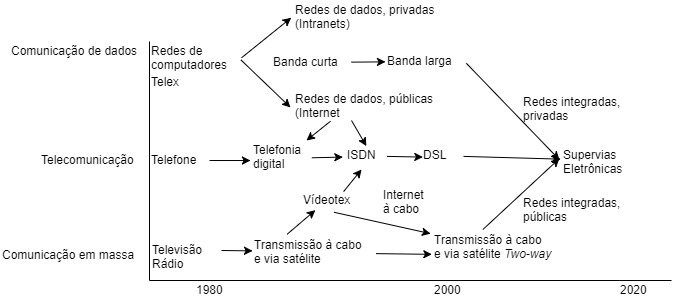
\includegraphics[width=.90\linewidth]{figuras/integrationoftransmission.jpg}
	\captionof{figure}{A integração das transmissões na comunicação. Adaptado de \cite[p.~7]{vandijk2006}.}
	\label{img:convergenciamidias}
\end{center}

\subsubsection{Convergência de terminais ou dispositivos}

Esta convergência refere-se a como a digitização consolida a centralização de vários dispositivos de mídia em um. \cite[p.~2]{storsul2010} ratificam que o cenário onde vários dispositivos são fundidos e suas funcionalidades são adicionadas em um só, se tornou realidade nas últimas décadas, porém o capitalismo retém a criação de um super dispositivo centralizador, pois está crescendo o número de terminais criados para tipos de mídia específicos, que vai na contramão da convergência.

\subsubsection{Convergência de serviços}

Com a convergência das redes e dos terminais iniciou-se o uso de diversos serviços nesses terminais, portanto era esperado a convergência dos serviços. Como retratam \cite{storsul2010} com a integração dos terminais e a capacidade de mandar qualquer tipo de informação por qualquer rede os serviços se tornariam mais integrados uns com os outros, ocasionando o surgimento de serviços multimídia. 

Os autores citam que os serviços integrados de televisão, como programas onde se pode interagir via e-mail ou por outras tecnologias diretamente na tela do televisor e serviços audiovisuais largamente difundidos na internet, estão ganhando terreno, e isso se deve ao fato da digitização do setor, que permite a convergência dos serviços.

\subsubsection{Convergência de mercado}

Com as convergências das infra-estruturas, dos terminais e dos serviços acontecendo, o mercado provavelmente responderia à mudança se tornando mais central com a digitização desse setores. \cite{storsul2010} denotam ainda como a convergência dos mercados deu início à economia de mídia. Não teriam limites bem definidos entre serviços e infra-estruturas e entre software e conteúdo de mídia. Portanto, surgiram alianças entre as companhias de tecnologia da informação e comunicação, telecom e de mídia originando novas empresas com foco em vários campos, as companhias multimídia.

\subsection{Definição dos serviços digitizados}

Existe uma diferença entre os tipos de convergência e os significados de digitização e digitalização. Os serviços digitizados, portanto, são resultados das convergências de várias tecnologias esperando fornecer algo ao consumidor de forma simples, rápida e integrada com os meios tecnológicos atuais. Lembrando que os conceitos básicos de serviços ainda são mantidos quando são transicionados para sua forma digital, com a adição das convergências de tecnologia e utilização da digitalização de documentos e processos. 

Desta forma, podemos avançar na descrição de como o serviço digitizado pode ser avaliado sob a ótica dos meios onde são viabilizados.

